\documentclass{article}
\usepackage{amsmath}
\usepackage{amsfonts}
\usepackage{physics}
\usepackage{amssymb}
\usepackage{booktabs} % For formal tables
\usepackage{graphicx}
\usepackage{empheq}

\begin{document}

\section*{PROBLEMS:}

\subsection*{Problem 5}
Now let's confront our estimates in problem 4 (problem set 1) with experiment.

\subsubsection*{(a) Question}
Make a simple table comparing your variational bounds with the observed ground state energies for lithium, beryllium, and nitrogen. Note that a simple web search for ``ionization potentials'' will get you a multitude of tables of observed values, or you can look at a reference such as the CRC Press's \textit{Handbook of Chemistry and Physics}. The table entries are typically of the form:
\begin{equation*}
    B(Z, N) - B(Z, N - 1).
\end{equation*}

\subsubsection*{(a) Answer}
\begin{table}[h!]
\centering
\begin{tabular}{lccc}
\toprule
Element & Variational Bound (eV) & Observed Energy (eV) & Difference (eV) \\
\midrule
Lithium    & 33.6813 & 5.3917 & 28.2896 \\
Beryllium  & 45.4749 & 9.3227 & 36.1522 \\
Nitrogen   & 87.868 & 14.5341 & 73.3339 \\
\bottomrule
\end{tabular}
\caption{Comparison of Variational Bounds with Observed Ground State Energies}
\label{tab:comparison}
\end{table}

\subsubsection*{(b) Question}
Do your results make sense? If not, can you figure out what is wrong, and whether the calculation we did for He is to be trusted?

\subsubsection*{(b) Answer}
My results don't make sense, they are way too large consistently. However, my calculation for He is to be trusted, as I obtained a variational bound for one spatial orbital. Since you can have He's two electrons of opposite spin in the same spatial orbital, this doesn't violate the Pauli exclusion principle. However, for the other elements with more electrons, you are fitting more than two electrons into the same spatial orbital, and this is not allowed by the Pauli exclusion principle.

\subsection*{Problem 6}
When we discussed the WKB method, we used the fact that if the potential was a constant, the phase of the wave function depended on \( x \) according to \( p(x) = \sqrt{2m(E-V)}\; \text{if}\; \phi(x = 0) = 0 \). Allowing the potential to slowly vary with \( x \), we computed the change in phase from \( x = x_0 \) to \( x \) as
\begin{equation}
    \phi(x) = \int_{x_0}^{x} \sqrt{2m(E-V)}\,dx.
\end{equation}

Thus, if the potential is slowly varying (such that the main variation of the wave function is due to the phase variation), we can write the wave function at \( x \) in terms of the wave function at \( x_0 \) approximately by
\begin{equation}
    \psi(x) \approx \psi(x_0) \exp \left\{ i \int_{x_0}^{x} \sqrt{2m(E-V(x'))}\,dx' \right\}.
\end{equation}

The WKB approximation may be used to estimate tunneling rates through a barrier. That is, there may be a region of potential greater than the energy between two regions where the potential is smaller than the energy. If the particle is in one of the ``allowed'' regions, it cannot classically penetrate the barrier, but it can according to quantum mechanics. Let us consider an example.



% The figure will be included here in the LaTeX document
% Replace 'figure.png' with the actual file name of the figure
\begin{figure}[h!]
    \centering
    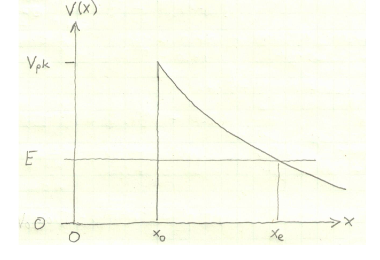
\includegraphics[width=0.6\textwidth]{figure.png}
    \caption{Potential \( V(x) \) as a function of \( x \) with labels for \( V_{pk} \), \( E \), and \( x_0 \).}
\end{figure}

We use the WKB method to estimate the tunneling rate as follows: We imagine the \( \alpha \) particle is bound in the nucleus, between \( x = 0 \) and \( x = x_0 \). Sometimes it bounces up against the potential barrier at \( x = x_0 \). When this occurs, there is some probability that it will escape the nucleus, where this probability is just \( |\psi(x_e)/\psi(x_0)|^2 \), where the wave function is estimated according to the WKB method in Eq. 2.

In the classically forbidden region between \( x = x_0 \) and \( x = x_e \), the ``phase'' is imaginary, and the exponential factor damps the wave function according to \( e^{-\Delta/2} \), where
\begin{equation}
    \Delta/2 = \int_{x_0}^{x_e} \sqrt{2m\lvert V(x') - E \rvert}\,dx'.
\end{equation}

\subsubsection*{(a) Question}
Find an expression for \( \Delta \) by evaluating this integral. It will be convenient to use the ratio \( \rho = x_0/x_e \). Try to simplify as much as you can. Note that you may find the discussion in the text on pages 444-445 helpful.

After emitting the \( \alpha \) particle, the daughter nucleus has a charge of \( Z_1 - 2 \). Thus, we have:
\begin{equation}
    V(x) = \frac{(Z_1 - 2)Z_2e^2}{4\pi \epsilon_0 x}
\end{equation}
where \( Z_1 = 92 \) and \( Z_2 = 2 \). Thus, we have:
\begin{equation}
    V(x) = \frac{180e^2}{4\pi \epsilon_0 x}
\end{equation}
Let's define:
\begin{equation}
    \beta = \frac{180e^2}{4\pi \epsilon_0}
\end{equation}
So:
\begin{equation}
    V(x) = \frac{\beta}{x}
\end{equation}
And we have:
\begin{equation}
    V(x_e) = E
\end{equation}
So, we have:
\begin{align}
    \frac{\beta}{x_e} &= E \\
    x_e &= \frac{\beta}{E}
\end{align}
So, we want to integrate:
\begin{equation}
    \Delta/2 = \int_{x_0}^{x_e} \sqrt{2m\lvert \frac{\beta}{x'} - E \rvert}\,dx'
\end{equation}
My script gives:
\begin{equation}
    \Delta = 2
\end{equation}
\subsubsection*{(a) Answer}
% Insert your answer here

\subsubsection*{(b) Question}
Find an expression for \( x_e \) in terms of known quantities.

\subsubsection*{(b) Answer}
% Insert your answer here

\subsubsection*{(c) Question}
To estimate the decay rate, we must multiply the tunneling probability by the rate at which the \( \alpha \) strikes the potential barrier at \( x_0 \). For this rate to strike the barrier by estimating the speed of the \( \alpha \) particle and the distance traveled between collisions.

\subsubsection*{(c) Answer}
% Insert your answer here

\subsubsection*{(d) Question}
Finally, put it all together and obtain a numerical prediction for the uranium decay rate. If the known hourly rate compares the speed of the \( \alpha \) particle to travel the barrier by obtaining the actual prediction and using the distance traveled between collisions.

\subsubsection*{(d) Answer}
% Insert your answer here

\subsection*{Problem 7}
Let's do a very simple calculation using the Ritz method, in order to make sure we understand the idea. Suppose we are interested in the energy levels of a particle of mass \( m \) in the one dimensional potential:
\begin{equation}
    V(x) = \begin{cases}
    0 & x \in (-L/2, L/2) \\
    \infty & \text{otherwise}
    \end{cases}
\end{equation}
Of course, we know the exact answer to both the eigenstates and eigenvalues for this system. However, let us pretend that we don't, and try using the Ritz method to estimate the two lowest energy levels. Thus, let us pick two trial wave functions. We might by accident in this simple case actually pick the exact functions, but we'll avoid that. Let us make an ``educated guess'', and choose:
\begin{align}
    |1\rangle &= A_1 \left[ (L/2)^2 - x^2 \right] \\
    |2\rangle &= A_2 x \left[ (L/2)^2 - x^2 \right],
\end{align}
where \( A_1 \) and \( A_2 \) are normalization constants and it is understood that these functions are taken to be zero when \( |x| \geq L/2 \). I encourage you to consider why this might be a good guess, even if we avoided the exact answers.

\subsubsection*{(a) Question}
Carry out the Ritz procedure using these two trial wave functions, and estimate the two lowest energy levels. Along the way, try to note how we really did make some good choices.

\subsubsection*{(a) Answer}
Our expansion looks like the following:
\begin{equation}
    \ket{\psi} = c_1\ket{1} + c_2\ket{2}
\end{equation}
where
\begin{equation}
    |c_1|^2 + |c_2|^2 = 1
\end{equation}
We first set out to normalize our trial wave functions:
\begin{align}
    \braket{1}{1} = 1 &= \int_{-L/2}^{L/2} A_1^2 \left[ (L/2)^2 - x^2 \right]^2 dx \\
\end{align}
My attached script in Sympy gives:
\begin{equation}
\boxed{A_1 = \left(\frac{30}{L^5}\right)^{1/2}}
\end{equation}
Next, we normalize the other one:
\begin{align}
    \braket{2}{2} = 1 &= \int_{-L/2}^{L/2} A_2^2 x^2 \left[ (L/2)^2 - x^2 \right]^2 dx \\
\end{align}
My attached script in Sympy gives:
\begin{equation}
\boxed{A_2 = 2\left(\frac{210}{L^7}\right)^{1/2}}
\end{equation}
Now come we want to evaluate the functional for the energy:
\begin{equation}
    E(c_1, c_2) = \bra{\psi}H\ket{\psi} = c_1^*c_1\bra{1}H\ket{1} + c_2^*c_2\bra{2}H\ket{2} + c_1^*c_2\bra{1}H\ket{2} + c_2^*c_1\bra{2}H\ket{1}
\end{equation}
with the Hamiltonian:
\begin{equation}
    H = -\frac{\hbar^2}{2m}\frac{d^2}{dx^2}
\end{equation}
Now, we evaluate the matrix elements:
\begin{align}
    \bra{1}H\ket{1} &= \int_{-L/2}^{L/2} A_1^2 \left[ (L/2)^2 - x^2 \right] \left(-\frac{\hbar^2}{2m}\frac{d^2}{dx^2}\right) \left[ (L/2)^2 - x^2 \right] dx \\ &= \frac{A_1^2L^3\hbar^2}{6m}
\end{align}
\begin{align}
    \bra{2}H\ket{2} &= \int_{-L/2}^{L/2} A_2^2 x^2 \left[ (L/2)^2 - x^2 \right] \left(-\frac{\hbar^2}{2m}\frac{d^2}{dx^2}\right) \left[ (L/2)^2 - x^2 \right] dx \\ &= \frac{A_2^2L^5\hbar^2}{40m}
\end{align}
However, the other two matrix elements are zero. Thus, we have:
\begin{equation}
    E(c_1, c_2) = \frac{A_1^2L^3\hbar^2}{6m}|c_1|^2 + \frac{A_2^2L^5\hbar^2}{40m}|c_2|^2
\end{equation}
Now, we want to use the Lagrange multiplier method to find the minimum of this functional. Thus, we define the Lagrangian:
\begin{equation}
    \mathcal{L} = E(c_1, c_2) - \lambda(|c_1|^2 + |c_2|^2 - 1)
\end{equation}
We take the partial derivatives with respect to $c_1^*$, $c_2^*$, and $\lambda$ and set them equal to zero:
\begin{align}
    \frac{\partial \mathcal{L}}{\partial c_1^*} &= \frac{A_1^2L^3\hbar^2}{6m}c_1 - \lambda c_1 = 0 \\
    \frac{\partial \mathcal{L}}{\partial c_2^*} &= \frac{A_2^2L^5\hbar^2}{40m}c_2 - \lambda c_2 = 0 \\
    \frac{\partial \mathcal{L}}{\partial \lambda} &= |c_1|^2 + |c_2|^2 - 1 = 0
\end{align}
Now, we wish to solve this system of equations. We first solve for $\lambda$:
So, we have:
\begin{align}
    \frac{A_1^2L^3\hbar^2}{6m}c_1 &= \lambda c_1 \\
    \frac{A_2^2L^5\hbar^2}{40m}c_2 &= \lambda c_2 \\
    |c_1|^2 + |c_2|^2 &= 1
\end{align}


\subsubsection*{(b) Question}
Compare your results with the exact eigenvalues for the two lowest levels.

\subsubsection*{(b) Answer}
% Insert your answer here

\subsection*{Problem 8}
Consider an ``anharmonic'' oscillator, in which we add a perturbation
\begin{equation}
    V = -\rho \omega \hat{X}^3.
\end{equation}
to the one-dimension harmonic oscillator Hamiltonian. Here, we define $ \hat{X} = \sqrt{m\omega}X$. The unperturbed Hamiltonian is
\begin{equation}
    H_0 = \frac{P^2}{2m} + \frac{m\omega^2 X^2}{2}.
\end{equation}
The parameter \( 0 < \rho \ll 1 \) is a small dimensionless parameter giving the strength of the perturbation. [We assume that the perturbation is sufficiently small that we needn't worry about what happens at very large values of \( x \).]

\subsubsection*{(a) Question}
Write the perturbation in terms of the raising and lowering operators \( a \) and \( a^\dagger \). Compute all of the non-zero matrix elements of \( V \) in the basis of the unperturbed eigenstates.

\subsubsection*{(a) Answer}
First, we note that:
\begin{equation}
    X = \sqrt{\frac{\hbar}{2m\omega}}(a + a^\dagger).
\end{equation}
so that:
\begin{equation}
    \hat{X} = \sqrt{\frac{\hbar}{2}}(a + a^\dagger).
\end{equation}
Then, we have:
\begin{align}
    V &= -\rho \omega \hat{X}^3 \\
    &= -\rho \omega \left( \sqrt{\frac{\hbar}{2}}(a + a^\dagger) \right)^3 \\
    &= -\rho \omega \left( \sqrt{\frac{\hbar}{2}} \right)^3 (a + a^\dagger)^3 \\
    &= -\rho \omega \left( \sqrt{\frac{\hbar}{2}} \right)^3 (a^3 + 3a^2a^\dagger + 3aa^{\dagger 2} + a^{\dagger 3}) \\
    &= -\rho \omega \left(\frac{\hbar}{2}\right)^{3/2} (a^3 + 3a^{\dagger 2}a + 3a^{\dagger}a^2 + a^{\dagger 3}).
\end{align}
Let us define $V'$:
\begin{equation}
    V' = a^3 + 3a^{\dagger 2}a + 3a^{\dagger}a^2 + a^{\dagger 3}
\end{equation}
In the basis of unperturbed eigenstates, only the $\ket{n+3}$, $\ket{n+1}$, $\ket{n-1}$, and $\ket{n-3}$ states have non-zero matrix elements. Thus, following this order, we have:
\begin{align}
    \bra{n}V'\ket{n+3} = \bra{n}a^3\ket{n+3} = \sqrt{(n+3)(n+2)(n+1)} \\ \implies \boxed{\bra{n}V\ket{n+3} = -\rho \omega \left(\frac{\hbar}{2}\right)^{3/2} \sqrt{(n+3)(n+2)(n+1)}} \\
\end{align}
Next, we have:
\begin{align}
    \bra{n}V'\ket{n+1} = \bra{n}3a^{\dagger}a^2\ket{n+1} = 3\sqrt{n^2(n+1)} \\ \implies \boxed{\bra{n}V\ket{n+1} = -3\rho \omega \left(\frac{\hbar}{2}\right)^{3/2} \sqrt{n^2(n+1)}} \\
\end{align}
Next, we have:
\begin{align}
    \bra{n}V'\ket{n-1} = \bra{n}3a^{\dagger 2}a\ket{n-1} = 3\sqrt{n(n-1)^2} \\ \implies \boxed{\bra{n}V\ket{n-1} = -3\rho \omega \left(\frac{\hbar}{2}\right)^{3/2} \sqrt{n(n-1)^2}} \\
\end{align}
Finally, we have:
\begin{align}
    \bra{n}V'\ket{n-3} = \bra{n}a^{\dagger 3}\ket{n-3} = \sqrt{n(n-1)(n-2)} \\ \implies \boxed{\bra{n}V\ket{n-3} = -\rho \omega \left(\frac{\hbar}{2}\right)^{3/2} \sqrt{n(n-1)(n-2)}} \\
\end{align}
\subsubsection*{(b) Question}
Compute the perturbed energy levels to the lowest non-trivial order in the perturbation.

\subsubsection*{(b) Answer}
The first order energy convection would indeed be trivial, as $E^{(1)} = \bra{n}V\ket{n} = 0$. Thus, we must compute the second order energy correction:
\begin{align}
    E^{(2)}_n &= \sum_{m \neq n} \frac{\lvert \bra{m}V\ket{n} \rvert^2}{E_n^{(0)} - E_m^{(0)}} \\
    &= \frac{\lvert \bra{n+3}V\ket{n} \rvert^2}{E_n^{(0)} - E_{n+3}^{(0)}} + \frac{\lvert \bra{n+1}V\ket{n} \rvert^2}{E_n^{(0)} - E_{n+1}^{(0)}} + \frac{\lvert \bra{n-1}V\ket{n} \rvert^2}{E_n^{(0)} - E_{n-1}^{(0)}} + \frac{\lvert \bra{n-3}V\ket{n} \rvert^2}{E_n^{(0)} - E_{n-3}^{(0)}} \\
    &= \frac{\rho^2 \omega^2 \hbar^3}{8} \left[ \frac{(n+3)(n+2)(n+1)}{E_n^{(0)} - E_{n+3}^{(0)}} + \frac{3n^2(n+1)}{E_n^{(0)} - E_{n+1}^{(0)}} + \frac{3n(n-1)^2}{E_n^{(0)} - E_{n-1}^{(0)}} + \frac{n(n-1)(n-2)}{E_n^{(0)} - E_{n-3}^{(0)}} \right] \\
\end{align}
We know that:
\begin{equation}
    E_n^{(0)} = \hbar \omega \left( n + \frac{1}{2} \right)
\end{equation}
Thus, we have:
\begin{align}
    E^{(2)}_n &= \frac{\rho^2 \omega^2 \hbar^3}{8} \left[ \frac{(n+3)(n+2)(n+1)}{-3\hbar \omega} + \frac{3n^2(n+1)}{-\hbar \omega} + \frac{3n(n-1)^2}{\hbar \omega} + \frac{n(n-1)(n-2)}{3\hbar \omega} \right] \\
    &= \frac{\rho^2 \omega \hbar^2}{8} \left[ \frac{(n+3)(n+2)(n+1)}{-3} - 3n^2(n+1) + 3n(n-1)^2 + \frac{n(n-1)(n-2)}{3} \right] \\
    &= \frac{\rho ^2 \omega \hbar^2}{8}\left[ -12n^2 -2\right]\\
    &= \boxed{-\frac{\rho ^2 \omega \hbar^2}{2}\left[ 3n^2 + \frac{1}{2}\right]}
\end{align}

\subsubsection*{(c) Question}
Compute the perturbed energy eigenfunctions to the lowest non-trivial order in the perturbation. Express in terms of the unperturbed energy eigenfunctions.

\subsubsection*{(c) Answer}
We have:
\begin{equation}
    \ket{N}= \ket{n} - \sum_{m \neq n} \frac{\bra{m}V\ket{n}}{E_n - E_m} \ket{m}
\end{equation}
We expand equation 38 with the elements of the summation that survive:
\begin{align}
    \ket{N} &= \ket{n} - \frac{\bra{n+3}V\ket{n}}{E_n - E_{n+3}} \ket{n+3} - \frac{\bra{n+1}V\ket{n}}{E_n - E_{n+1}} \ket{n+1} - \frac{\bra{n-1}V\ket{n}}{E_n - E_{n-1}} \ket{n-1} - \frac{\bra{n-3}V\ket{n}}{E_n - E_{n-3}} \ket{n-3} \\
    &= \ket{n} - \frac{-\rho \omega \left(\frac{\hbar}{2}\right)^{3/2} \sqrt{(n+3)(n+2)(n+1)}}{\hbar \omega \left( n + \frac{1}{2} - (n+\frac{5}{2})\right)} \ket{n+3} - \frac{-3\rho \omega \left(\frac{\hbar}{2}\right)^{3/2} \sqrt{n^2(n+1)}}{\hbar \omega \left( n + \frac{1}{2} - (n+\frac{3}{2})\right)} \ket{n+1} \\
    &- \frac{-3\rho \omega \left(\frac{\hbar}{2}\right)^{3/2} \sqrt{n(n-1)^2}}{\hbar \omega \left( n + \frac{1}{2} - (n-\frac{1}{2})\right)} \ket{n-1} - \frac{-\rho \omega \left(\frac{\hbar}{2}\right)^{3/2} \sqrt{n(n-1)(n-2)}}{\hbar \omega \left( n + \frac{1}{2} - (n-\frac{3}{2})\right)} \ket{n-3} \\
\end{align}
We simplify:
\begin{empheq}[box=\fbox]{align}
\begin{split}
\ket{N} &= \ket{n} - \frac{\rho\sqrt{\hbar(n+3)(n+2)(n+1)}}{2\sqrt{2}} \ket{n+3} \\
&\quad - \frac{3\rho\sqrt{\hbar n^2(n+1)}}{\sqrt{2}} \ket{n+1} \\
&\quad + \frac{3\rho\sqrt{\hbar n(n-1)^2}}{\sqrt{2}} \ket{n-1} \\
&\quad + \frac{\rho\sqrt{\hbar n(n-1)(n-2)}}{2\sqrt{2}} \ket{n-3}
\end{split}
\end{empheq}



\end{document}
